\chapter{The Correct Usage of ...}


\section{Footnotes}

Footnotes were invented by the humanities, where dealing with research sources is of high
significance. Footnotes here mainly serve as references to the source of a citation.
In the field of computer science, however, footnotes are \textbf{used rather scarcely}.
If a reference to an external source is required, the source will be referenced (see
chapter \ref{sec:references}).

Footnotes are often used for remarks that are not supposed to appear within the 
actual text. However, if the remark is important enough to be mentioned, it 
can as well be placed in the main text. Otherwise it is probably not that important
and we can do witout it.  \footnote{Do you realize how this meaningless footnote
  obstructs the read flow?}


\section{Page Numbers}

Page numbers are important for the simple reason that the printed document is not
always stapled when it lies on a desk, and a draft through the open door is
sometimes enough to sweep the whole stack off the desk and turn it upside down.
In addition, page numbers are very helpful in the process of reviewing ("The first
paragraph on page 67 should be rephrased"). Therefore, we recommend to \textbf{always
  use page numbers}.


\section{Figures}

Figures are meant to improve the comprehensibility of the text and should therefore
be \textbf{generously applied} (mind that "generously" must not be taken
too literal). According to our experience, an average of one figure in \textbf{2-3 pages}
is acceptable. Too many figures would cause the impression of a comic strip.

A figure says more than a thousand words, however, it can not replace descriptive
comments in the text. A general rule says that a figure should support the comprehension
of a text, but by no means can be planted into it without further explanation.
It is important to always make sure that the text provides \textbf{references and descriptions} 
to the figures. In addition, each figure should be captioned in an explanatory way.

\begin{quotation}

  \begin{figure}
    \begin{center}
      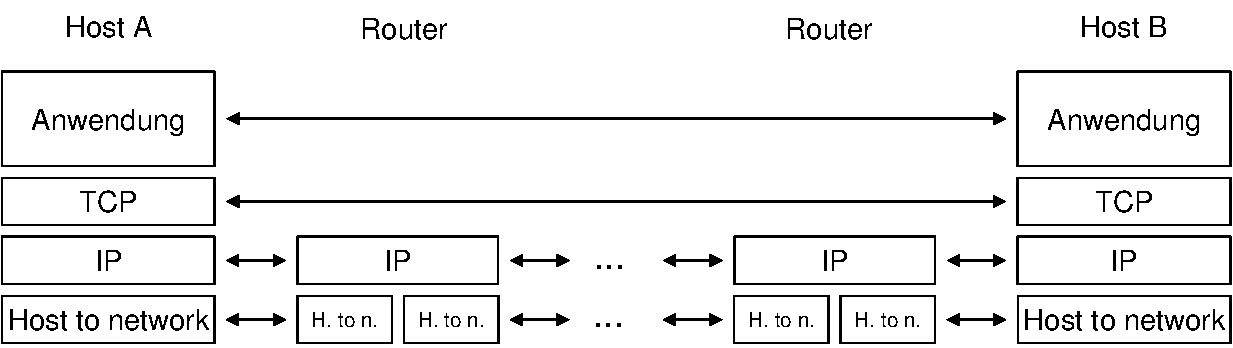
\includegraphics[width=\textwidth]{fig/communication}
      \caption{The TCP/IP protocol stack during the communication process 
        between two hosts}
      \label{fig:1}
    \end{center}
  \end{figure}
  
  \fbox{
    \begin{minipage}{.876\textwidth}
      \subsubsection*{Example}
      
      TCP and IP have different functions. Figure \ref{fig:1} shows the 
      interaction of both protocols during the communication of the two
      nodes A and B that are interconnected via several routers. IP, being
      the protocol analog to the third layer in the OSI-Model, has the
      function of ... \emph{(... continue discussion of the figure)}
     \end{minipage}
  }
\end{quotation}

  
\subsection*{Figures of Other Authors}

Lots of figures have been created, among them may even be figures that
exactly match your work. If you find such a figure, you might want to use
it in your paper/thesis. In this case you have to make a \textbf{figure reference}
to the source of the figure; either in the figure itself or in the annex.

If you wish to use a figure that is not available in an electronic format,
the simplest of all solutions is to scan it. If the figure is part of an 
electronic document, you can make a screenshot. Mind that, using this type
of figures, it is important to choose a sufficiently high resolution to ensure
that the printer will not turn it into a load of "pixel mud".
At the same time, the resolution should be as low as possible in order to not
unecessarily blow up the size of the document.

Therefore, it is worth considering to draw the picture yourself with a tool
of your own preference and embed it as a \textbf{vector graphics}.  
In most of the cases you will end up having to apply changes to a foreign figure,
because it eventually turns out to not 100\% match with the situation in your work.
If after that the figure still strongly resembles the source, and if it is not a
commonly well-known picture, as e.g. the TCP/IP protocol stack, the source must
be marked as "according to [reference]". We recommend to choose
a vector format (.wmf, .emf, .eps, .pdf), since they do not occupy much space
and scale arbitrarily without looking "pixelish".


\subsection*{Colors}

A colored figure is a nice thing - provided you will use a color printer. In a
black-and-white-print the colors will be reduced to their grades of brightness, as
a result of which the contrast distribution will not remotely reach the intended
quality. Therefore, when creating colored figures, make sure that even in a black-and-white
print the necessary information will still be distinct. You can as well abstain
from colors and use different shades of gray instead. In plots, different curves can
be distinguished by using different line types.

However, if you wish to use colored figures, do not refer to the colors in the text.
Phrases like "Active nodes are marked red, passive nodes blue and inactive nodes green"
in a black-and-white print have a rather comical effect and will lead to confusion rather 
than comprehension.


\subsection*{Plots}

Plots should be created e.g. with Gnuplot \cite{gnuplot_homepage}, R \cite{r_homepage},
OpenOffice \cite{oo_homepage}, or Excel. They can easily be embedded as vector formats,
so it is not necessary to use screen shots. When using plots, it is important to \textbf{label the
axes} and indicate the \textbf{units}.

Make sure to use an \textbf{appropriate scaling}. For example, instead of saying "10000000 bps"
or "1.0e-07 bps" the more concise "10 Mbps" is preferable.

An example of how not to do it is shown in figure \ref{fig:plots} (a): a pixelish Gnuplot-screenshot
without units at the axes and a badly chosen scaling. Example (b) shows the same plot with
a reasonable labeling as .eps import.

\begin{figure}[htbp]
  \begin{center}
    \subfigure[Poor] {
      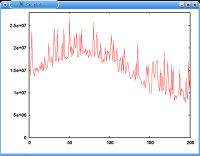
\includegraphics[width=10cm]{fig/plot_falsch_small}
    }
    \subfigure[Better] {
      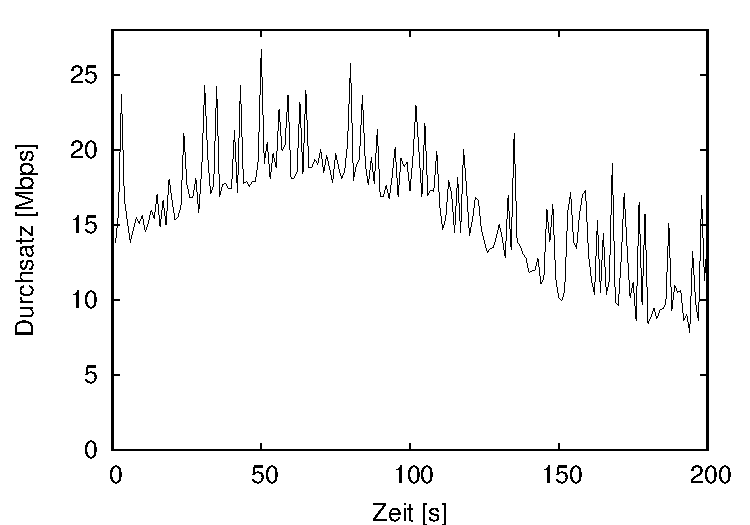
\includegraphics[width=10cm]{fig/plot_richtig}
    }
    \caption{Examples for a presentation of measurement results}
    \label{fig:plots}
  \end{center}
\end{figure}


\section{Tables}

The same rules that apply to figures also apply for tables:
Tables have to be numbered, captioned, and referenced in the text.


\begin{quotation}
  \fbox{
    \begin{minipage}{.876\textwidth}
      \subsubsection*{Example}
      
      To analyse the aspect XYZ, three test series were carried out
      in the test systems. Table \ref{tab:config} summarizes the
      sender- and receiver configurations used in the test series.
    \end{minipage}
  }
\end{quotation}

In case you wish to present extensive measurement- or simulation results, a graphic
representation could possibly convey the information more concisely than a table.


\begin{table}
  \renewcommand{\arraystretch}{1.5}
  \begin{center}
    \begin{tabular}{|c|c|c|}
      \hline
      \textbf{Test Series} & \textbf{Sender} & \textbf{Recipient} \\
      \hline
      1 & heineken & grolsch \\
      \hline
      2 & heineken & bitburger  \\
      \hline
      3 & grolsch & bitburger \\
      \hline
    \end{tabular}
    \caption{Sender- and recipient configurations of the implemented test series}
    \label{tab:config}
  \end{center}
\end{table}


\section{Quotations}
\label{sec:quotations}

We recommend to not extensively quote text sources. Computer scientists usually
make it short; instead of quoting a source, they reference it in the appropriate
place. However, it can be helpful to now and then quote a particular paragraph 
containing information which is crucial for your work. In this case, the quotation
has to be put in \textbf{quotation marks} and stand out against the rest of the
text (for example, by indented paragraphs or italicized font). Furthermore, the 
source has to be indicated by a reference (see quote from the DPO in chapter
\ref{sec:aufgaben-diplom}).

By no means quotations may be used to describe the basics of your work. Although
it is easy to find elaborate introductions to most subjects, it would by far miss
the purpose of your work to simply adopt them. On the contrary, they can be rather
incoungruous since they most probably will not confine themselves to the essentials
of this aspect of your work.

If, in addition, the reference to the quotation is missing, it means that the author
tries to pass off a foreign work as his own. This is called plagiarism and is
incompatible with the methods of academic work which, as a purpose of our lectures,
we want the students to acquire.

\textbf{If we identify a case of plagiarism, we will get very angry -
   sometimes angry to an extent that we will refuse the certificate, or grade the
   Master thesis as not passed.}


\section{References}
\label{sec:references}

\subsection{What do I reference?}

When choosing a source, it is of great importance to check its reliability.
Usually, the  books, articles of scientific magazines or conference proceedings,
standards, and other sources that we make available for you undergo a scientific
review to ensure a certain reliability.

Computer magazines, such as c't, iX etc., belong to a scientific twilight
zone. They do get reviewed, however, the reviews are editorial, not
scientific, hence they should be referenced for non-technical aspects only.
For example, you should \emph{not} reference a TCP/IP-tutorial from the c't or,
even worse, the Computer-Bild - more appropriate here would be a reference to books
or the relevant standards. However, in an introduction it is not at all out of
place to quote from an article about the commercial predominance of a new radio
communication standard and reference the sales figures for end devices mentioned
in the article.

You will need a good deal of scepticism when dealing with internet publications
(including, among others, seminar/study papers from other authors) that were not
obviously subject to review. You better avoid this kind of sources, since the
internet makes it quite easy to publish the most amazing nonsense. 


\subsection{How do I reference?}

Two different ways of referencing have been established. The first one are
found mainly in English publications: The references are simply bracketed and
serially numbered:

\begin{quotation}  
  \fbox{
    \begin{minipage}{.876\textwidth}     
      \subsubsection*{Example}
      In [1] we introduce an alternative mechanism for congestion control 
      which recognizes congestion by the increase of round trip time.
    \end{minipage}
  }
\end{quotation}

Alternatively, the signature of the reference consists of the initials
of the authors' last names and the last 2 digits of the year of publication.
This form of referencing is most customary in German publications:

\begin{quotation}  
  \fbox{
    \begin{minipage}{.876\textwidth}
      \subsubsection*{Example}
      
      In [JWL04] we introduce an alternative mechanism for congestion
      control which recognizes congestion by the increase of round
      trip time.
    \end{minipage}
  }
\end{quotation}

The following rules have proven useful for both notations:

\begin{itemize}
\item To prevent a signature from getting too long, only the first
  three authors will be mentioned. If there are more than three authors,
  this is indicated by a "+" behind the list of authors
  (e.g. [IML+01] for a paper published by Inamure, Montenegro, Ludwig,
  Gurtov, and Khafizov in 2001).
  Testtt
\item In case there is only one author, the first three letters of his
  last name will be indicated (e.g. [Hus01] for an article published by
  Geoff Huston in 2001).
  
\item If an author or a group of authors produced more than one publication
  in one year, the referenced publications of the same year will be distinguished
  by an attached lowercase letter (e.g. [Pos81a], [Pos81b]).
  
\item If there is no designated author or publisher (which can happen in case
  of standards), arbitrarily choose an explicit letter combination (e.g.[IEEE99]
  for an IEEE standard).

\end{itemize}

The references will be listed in a separate chapter at the end of the document.
Each reference appears as a separate entry in the following format:

\begin{tabbing}
  [Signature] \= author(s), title of publication, specification about magazine,
  conference, \\ \> book in which the source was published, page number (if possible),\\
  \> year of publication, ISBN.
\end{tabbing}

The information contained in the reference list has to be exhaustive enough to enable
the reader to find the source (in fact, without using Google or Citeseer).


\subsubsection*{Examples for RFCs/Standards:}
\begin{tabbing}
  {}[IEEE99] \= \kill \\
  {}[Pos81a] \> J. Postel, \emph{Internet Protocol}, September 1981, IETF, RFC
  791, Status: \\*
  \> Standard.\\
  {}[Pos81b] \> J. Postel, \emph{Transmission Control Protocol}, September
  1981, IETF, RFC 793,\\*
  \> Status: Standard.\\
  {}[IEEE99] \> IEEE Computer Society LAN MAN Standards Committee,
  \emph{Wireless LAN} \\*
  \> \emph{Medium Access Control (MAC) and Physical Layer (PHY)
  Specifications,} \\*
  \> \emph{IEEE Std 802.11}, 1999 Edition, Institute of Electrical and
  Electronics\\*
  \> Engineers (IEEE), 1999.
\end{tabbing}


\subsubsection*{Example for a Conference Paper}

\begin{tabbing}
  [JWL04] \= C. Jin, D. Wei, and S. Low, \emph{FAST TCP: Motivation,
  Architecture,} \\*
  \> \emph{Algorithms, Performance}, Proceedings of the 23rd Annual Joint
  Conference \\*
  \> of the IEEE Computer and Communications Societies, INFOCOM 2004,
  \\*
  \> March 2004.
\end{tabbing}


\subsubsection*{Example for a Journal Article}

\begin{tabbing}
  [Hus01] \= G. Huston, \emph{Analyzing the Internet's BGP Routing Table},
 The Internet\\*
 \> Protocol Journal 4 (2001), no. 1, pp 2-15.
\end{tabbing}


\subsubsection*{Example for a Web Site}

\begin{tabbing}
  [TCP03] \= Homepage of Tcptrace - a tool for TCP trace Analysis, \\*
  \> http://www.tcptrace.org, November 2003.
\end{tabbing}

In a web site reference it is obligatory to indicate the date of the reference,
since web sites are not usually static nor permanent.


\subsubsection*{Example for a Book}

\begin{tabbing}
  [Ste94] \= W. R. Stevens, \emph{TCP/IP Illustrated: The Protocols}, vol. 1,
  \\*
  \> ISBN 0-201-63346-9, Addition Wesley 1994.
\end{tabbing}


\subsection{BibTeX}

When using the \emph{BibTeX} addition to LaTeX, the signature is generated
automatically, and you do not have to bother about their formats. In BibTeX,
the references are managed in a separate .bib file, from which the necessary
references will be extracted and embedded into the document by the \texttt{bibtex}
command. References in BibTeX format are often available in the Web and save
a lot of work.


\section{Abbreviations}

Please note that abbreviations and full text must not be mixed. When introducing
an abbreviation for the first time, it should be written in full with the 
abbreviation attached in brackets. In the following text, only the abbreviation will
be used. Common abbreviations can be applied without introducing them in full
writing.

\begin{quotation}
  \fbox{
    \begin{minipage}{.876\textwidth}
      \subsubsection*{Example}      
      The \emph{Transmission Control Protocol} (TCP) offers a reliable,
      connection-oriented transport service. TCP was ... \emph{(from now on
      always use "TCP")}
    \end{minipage}
  }
\end{quotation}

If a document contains a large amount of different abbreviations, it might be
reasonable to summarize them in a list and attach it to the document.


\section{Headlines and Titles}

Headlines are not part of the text and therefore must not be interlaced with the text. 


\begin{quotation}
  \fbox{
    \begin{minipage}{.876\textwidth}
      \subsubsection*{Example (poor)}
      
      \textbf{2.6 The TCP/IP Reference Model}\\ consists of four protocol
      layers which are depicted in figure \ref{fig:1}.

      \subsubsection*{Example (better)}
      
      \textbf{2.6 The TCP/IP Reference Model}\\
      The TCP/IP Reference Model, which contains 4 layers, is depicted in figure \ref{fig:1}.
      
    \end{minipage}
  }
\end{quotation}

\section{Indices}

If the volume of a document exceeds approximately 15 pages, it is advisable to 
generate a table of contents, for which every reasonable text system offers supportive
tools. 

In voluminous documents, such as Master theses, separate indices of figures and tables
are recommended.


\section{Programming Code}

To quote and discuss a voluminous programming code is one of the most effective means of
boring your reader. In case you decide to introduce an algorithm, you will rather
use a Pseudocode representation that confines itself to explaining the main functions
of the algorithm. If a reader is interested in the implementation, they can refer to
the actual programming code. For discussing data structures, UML class diagrams have proven
quite useful.
